\documentclass{beamer}

\usepackage{showexpl}
\usepackage{graphicx}

\usetheme{Boadilla}

\title{Computer Workshop}
\subtitle{Git in a team}
\author{Dr.\ MalekiMajd}
\institute[IUST]{Iran University Of Science And Technology}
\date{13 Dey, 1402}

\begin{document}
\frame{\titlepage}

\begin{frame}{Outline}
    \tableofcontents
\end{frame}

\begin{frame}{Introduction}
    \begin{itemize}
        \item Now that we have learned how to use git, we can use it in a team.
        \item Git is most useful when working in a team. It allows you to work on the same project with your teammates at the same time.
        \item No more hassle of sending files back and forth via email or USB drive.
    \end{itemize}
\end{frame}

\section{Setting up the environment}

\begin{frame}{Is GitHub necessary?}
    \begin{itemize}
        \item You might end up asking yourself, is GitHub necessary?
        \item The answer is no. You can use git without GitHub.
        \item Even some companies use git without GitHub and have their own servers where they host their repositories.
    \end{itemize}
\end{frame}

\begin{frame}{Wait a minute!}
    \begin{itemize}
        \item But why do we use GitHub?
        \item GitHub is a platform that makes it easier to work with git.
        \item It provides a lot of features that make working with git easier.
        \item It also provides a lot of features that make working in a team easier.
    \end{itemize}
\end{frame}

\begin{frame}{Keep an eye out for more FOSS alternatives}
    \begin{itemize}
        \item GitHub is not the only platform that provides these features.
        \item There are a lot of FOSS alternatives that provide the same features.
        \item GitLab is one of them.
        \item GitLab is a FOSS alternative to GitHub.
        \item It provides the same features as GitHub.
        \item It also provides some features that GitHub does not provide.
    \end{itemize}
\end{frame}

\begin{frame}{Some other alternatives}
    \begin{itemize}
        \item GitLab
        \item Gitea
        \item GitKraken
        \item Codeberg
        \item Bitbucket
        \item notabug.org
        \item SourceHut
        \item Launchpad
        \item Tuleap
    \end{itemize}
\end{frame}

\begin{frame}{The Linux Kernel repository}
    \begin{itemize}
        \item The main repository of the Linux Kernel is hosted on kernel.org.
        \item It also contains a mirror of the repository on GitHub.
        \item Turns out Torvalds isn't really a fan of GitHub.
    \end{itemize}
\end{frame}

\begin{frame}{Setting up the environment}
    \begin{itemize}
        \item First, you need to create a GitHub account.
        \item Then you need to create a repository.
        \item You can create a repository by clicking on the \texttt{New} button in the top left corner of the screen.
        \item You can also create a repository by clicking on the \texttt{+} button in the top right corner of the screen.
    \end{itemize}
\end{frame}

\begin{frame}{Adding collaborators}
    \begin{itemize}
        \item You can add collaborators to your repository.
        \item Collaborators are people who can push to your repository.
        \item You can add collaborators by going to the \texttt{Settings} tab of your repository.
        \item Then you need to click on the \texttt{Manage access} button.
        \item Then you need to click on the \texttt{Invite a collaborator} button.
    \end{itemize}
\end{frame}

\section{Get to know the process}

\subsection{The GitHub flow}

\begin{frame}{The GitHub flow}
    \begin{itemize}
        \item The GitHub flow is a process that is used to work with git in a team.
        \item It is a process that is used by a lot of companies.
        \item It is a process that is used by a lot of open source projects.
        \item Likewise, it is a process that is used by a lot of FOSS projects.
    \end{itemize}
\end{frame}

\begin{frame}{The GitHub flow}
    To use the GitHub flow, you need to follow these steps:
    \begin{enumerate}
        \item Create a branch
        \item Make changes
        \item Create a pull request
        \item Review the changes
        \item Merge your pull request
        \item Delete your branch
    \end{enumerate}
\end{frame}

\subsection{Branches}

\begin{frame}{Create a branch}
    \begin{itemize}
        \item The first step is to create a branch.
        \item You can create a branch by clicking on the \texttt{Branch: main} button in the top left corner of the screen.
        \item Then you need to enter the name of the branch you want to create.
        \item Then you need to click on the \texttt{Create branch} button.
        \item You can also create a branch using the command line as we had mentioned before.
    \end{itemize}
\end{frame}

\subsection{Make changes}

\begin{frame}{Make changes}
    \begin{itemize}
        \item The next step is to make changes to your code.
        \item You can make changes to the branch you had created.
        \item Your branch is a safe place to make changes.
        \item If you make a mistake, you can easily revert it.
        \item The changes you make will not affect the main branch until your merge it.

        \begin{block}{Tip}
            Make a separate branch for each set of unrelated changes. This makes it easier for reviewers to give feedback. It also makes it easier for you and future collaborators to understand the changes and to revert or build on them.
        \end{block}

    \end{itemize}
\end{frame}

\begin{frame}{Making changes}
    \begin{itemize}
        \item Ideally, each commit contains an isolated, complete change. This makes it easy to revert your changes if you decide to take a different approach.
        \item For example, if you want to rename a variable and add some tests, put the variable rename in one commit and the tests in another commit.
        \item Later, if you want to keep the tests but revert the variable rename, you can revert the specific commit that contained the variable rename.
        \item If you put the variable rename and tests in the same commit or spread the variable rename across multiple commits, you would spend more effort reverting your changes.
    \end{itemize}
\end{frame}

\subsection{Pull requests}

\begin{frame}{Pull requests}
    You might be wondering, what is a pull request?
    \begin{itemize}
        \item Pull requests let you tell others about changes you've pushed to a branch in a repository on GitHub.
        \item Once a pull request is opened, you can discuss and review the potential changes with collaborators and add follow-up commits before your changes are merged into the base branch.
    \end{itemize}
\end{frame}

\begin{frame}{Pull requests}
    \begin{itemize}
        \item Pull requests can come from either topic branches within the same repository or from a branch in a fork of the original repository.
        \item If the pull request is coming from a fork, you can still push commits to the topic branch after you open the pull request.
        \item These new commits will be added to the pull request automatically.
    \end{itemize}
\end{frame}

\begin{frame}{Pull requests: Experience it yourself}
    \begin{itemize}
        \item Now that you know what a pull request is, you can create one.
        \item You can create a pull request by clicking on the \texttt{Pull requests} tab of your repository.
        \item Then you need to click on the \texttt{New pull request} button.
        \item Then you need to select the branch you want to merge into the main branch.
        \item Then you need to click on the \texttt{Create pull request} button.
    \end{itemize}
\end{frame}

\begin{frame}{Pull requests: See others}
    \begin{itemize}
        \item It is recommended to see other pull requests to get a better understanding of how they work.
        \item Proper pull requests \textbf{include a summary, what problem they solve, and how they solve it.}
    \end{itemize}
\end{frame}

\subsection{Issues}

\begin{frame}{Issues}
    A tool that is used to track bugs and feature requests is called an issue tracker.

    \begin{itemize}
        \item Issues are a great way to keep track of tasks, enhancements, and bugs for your projects.
        \item They're kind of like email—except they can be shared and discussed with the rest of your team.
        \item Most software projects have a bug tracker of some kind.
    \end{itemize}
\end{frame}

\begin{frame}{Issues section in GitHub}
    You might have noticed that every repository contains a section called \texttt{Issues}.
    \begin{itemize}
        \item This is a section where you can report bugs, request features, and discuss things.
        \item You can also use it to keep track of tasks.
        \item Don't forget to \textbf{Use descriptive titles and descriptions.}
    \end{itemize}
\end{frame}

\subsection{Reviewing changes}

\begin{frame}{Reviewing changes}
    \begin{itemize}
        \item Once you have created a pull request, you need to wait for someone to review your changes.
        \item You can also review other people's changes.
        \item You can review changes by going to the \texttt{Pull requests} tab of your repository.
        \item Then you need to click on the pull request you want to review.
        \item Then you need to click on the \texttt{Files changed} tab.
    \end{itemize}
\end{frame}

\begin{frame}{Requesting a review}
    \begin{itemize}
        \item You can request a review from someone by clicking on the \texttt{Reviewers} tab of your pull request.
        \item Then you need to click on the \texttt{Request review} button.
        \item Then you need to select the person you want to request a review from.
        \item Then you need to click on the \texttt{Request} button.
    \end{itemize}
\end{frame}

\begin{frame}{Request changes}
    GitHub allows you to request changes from someone.
    \begin{itemize}
        \item You can request changes from someone by clicking on the \texttt{Review changes} button.
        \item Then you need to click on the \texttt{Request changes} button.
        \item Then you need to click on the \texttt{Submit review} button.
    \end{itemize}
\end{frame}

\begin{frame}{Merging changes}
    \begin{itemize}
        \item Once your pull request has been reviewed, you can merge it.
        \item You can merge your pull request by clicking on the \texttt{Merge pull request} button.
        \item Then you need to click on the \texttt{Confirm merge} button.
        \item Then you need to click on the \texttt{Delete branch} button.
    \end{itemize}
\end{frame}

\section{The develop branch}

\begin{frame}{The develop branch}
    Some projects might have a develop branch, and they might not merge pull requests into the main branch directly.
    \begin{itemize}
        \item The develop branch is a branch that is used to develop new features.
        \item It is a branch that is used to test new features before they are merged into the main branch.
\end{itemize}
\end{frame}

\begin{frame}{A demonstration}
    \begin{figure}
        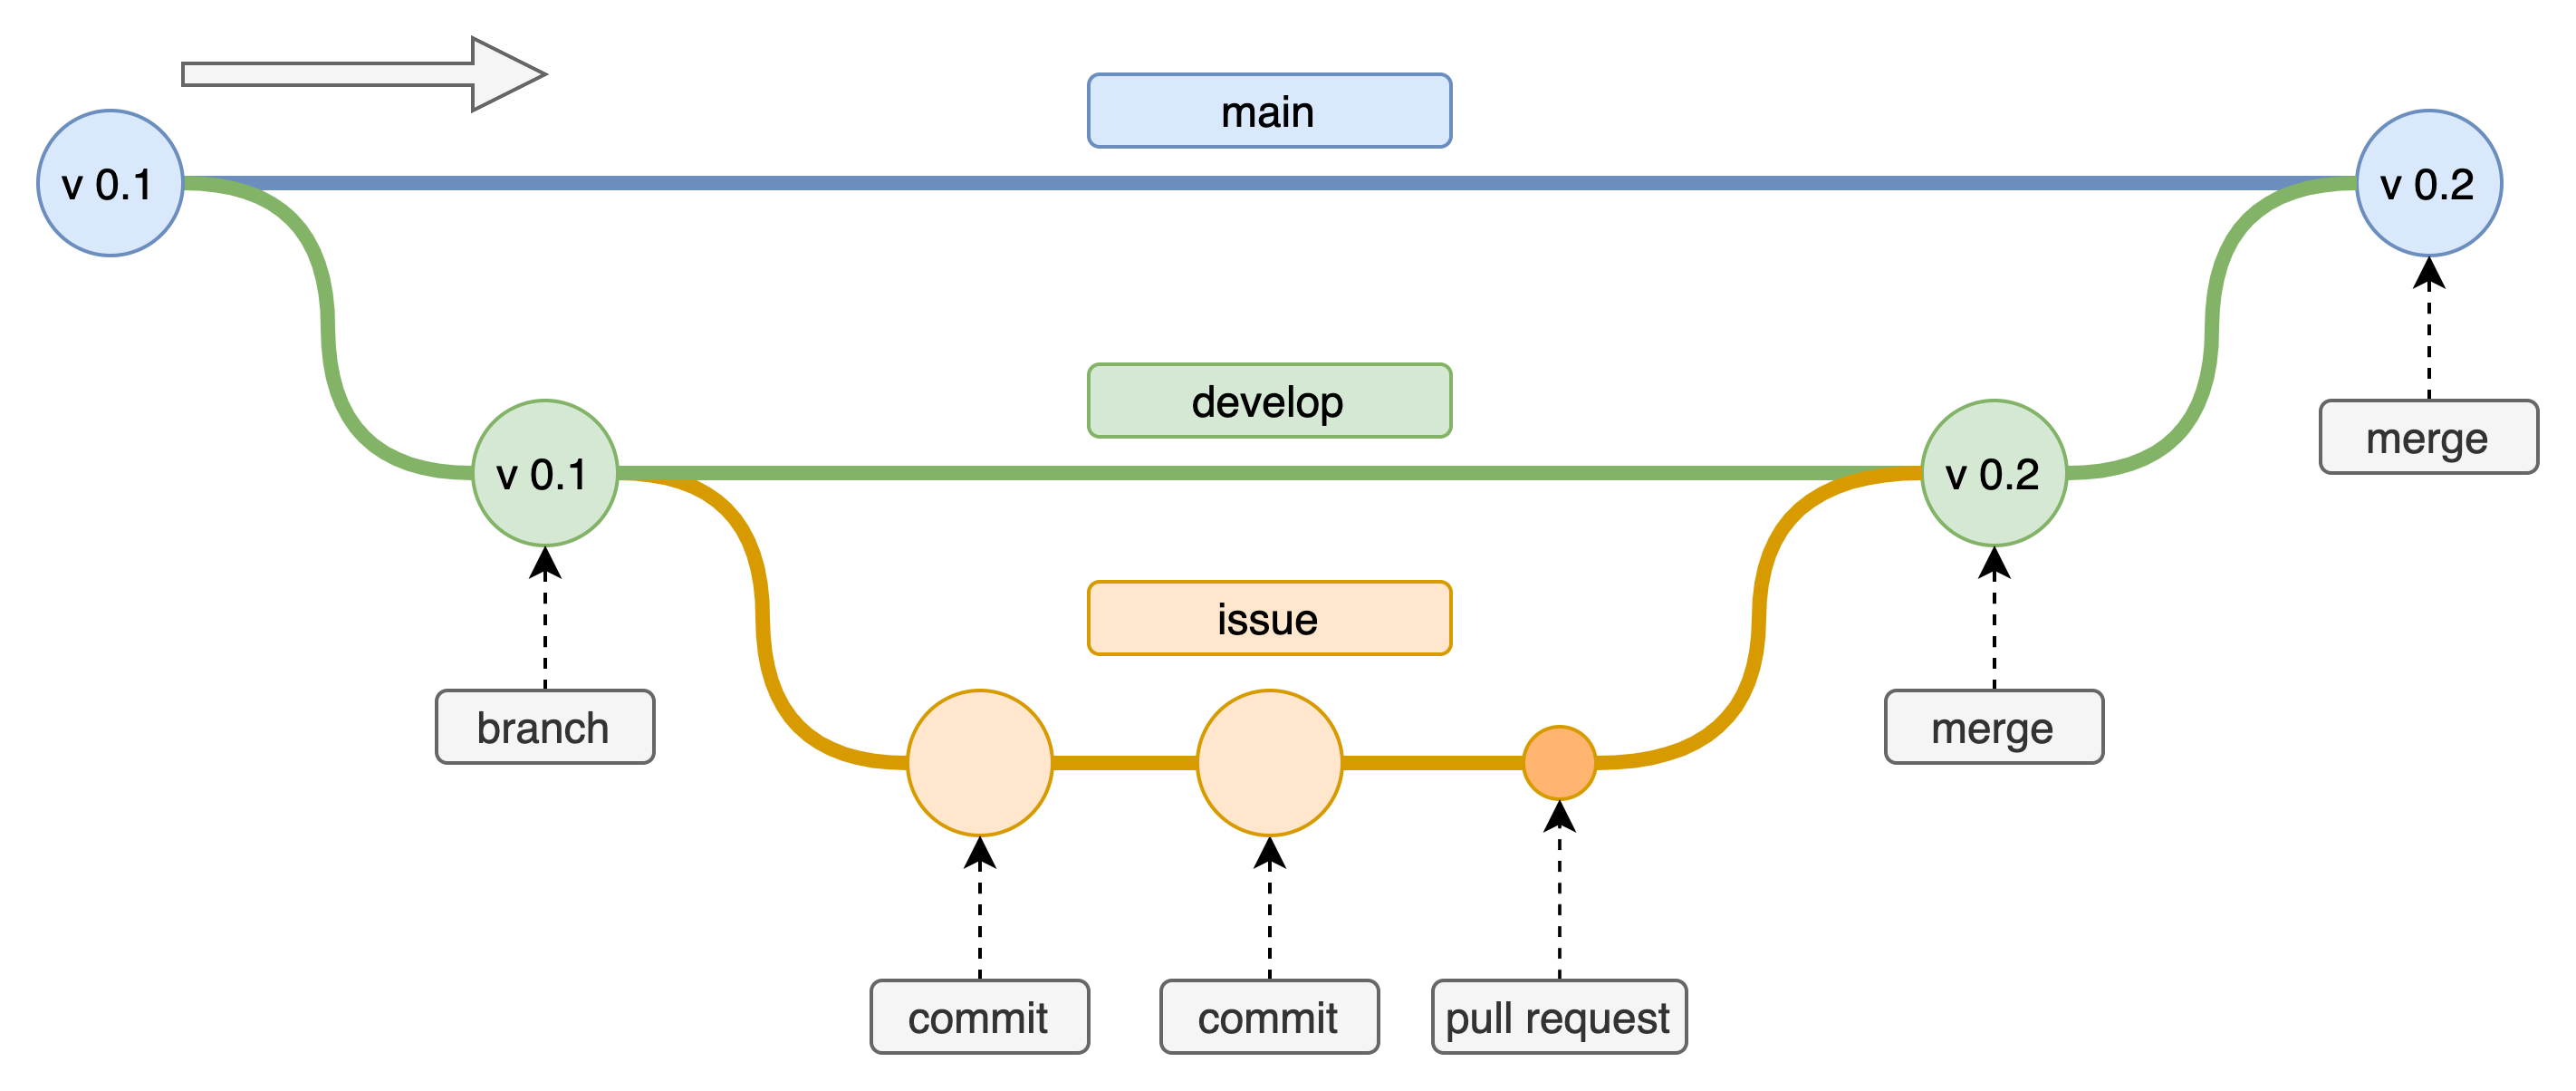
\includegraphics[width=\textwidth]{develop-branch.png}
        \caption{The develop branch}
    \end{figure}
\end{frame}

\begin{frame}{Feedback}
    \begin{center}
    Thanks for bearing with us for the last semester!
    \end{center}

    Any feedback is appreciated. Don't hesitate to contact me if you have any feedback/suggestions. Your feedback will help us improve the course.
\end{frame}

\end{document}